\subsubsection{Relationship typing}\label{sec:relationshiptype}

Stakeholders with different perspectives, goals and interests who are involved in software development may contribute to the capture and use of traceability information. Depending on their expertise and needs, they may come up with different types of traceability relations expressing different perspectives on the links among the elements in the project. It is very important to understand project specific conventions for interpreting the meaning of such relations~\cite{Spanoudakis2005} as their semantics will make any traceability analysis much richer and precise.

\begin{figure}[h]
	\centering
	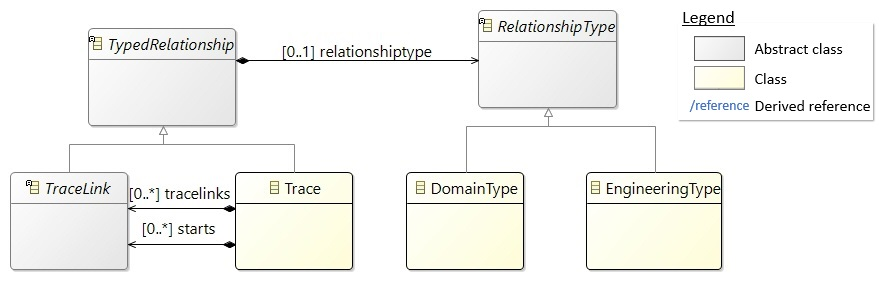
\includegraphics[width=.85\linewidth]{images/relationtyping.jpg}
	\caption{Customizable relationship types}
	\label{fig:mm-relation}
\end{figure}
As can be seen in Figure \ref{fig:mm-relation}, we refine the typing of relationships with a mechanism comparable to UML data typing~\cite{rumbaugh2004-UML2}. A \texttt{TypedRelationship} has an optional \texttt{RelationshipType}. A \texttt{RelationshipType} is abstract and specializes into different levels of sub types.
At the top level, \texttt{DomainType} and \texttt{EngineeringType} define predefined \texttt{RelationshipType}, without any substructure. 

On the one hand we have \texttt{DomainType} types coming from the application domain, used by experts of this domain. They convey semantics of the application domain. On the other hand, \texttt{EngineeringType} are types related to the engineering of software systems and focus on "how" artefacts are related (\textit{i.e.,} implements, Doc2Vec).  We aim to reflect in this architecture the cognitive gap that remains between traceability actors and the users of their product. 

This is an arbitrary separation and other specific types can be easily added to this general design, same as we had for the artefact types. As any metamodel, this one can also be extended to better suit the needs of a specific domain. Some of RelationshipTypes could be generic enough to be reused in different scenarios while others will be very scenario-specific.

\paragraph{Classes}
\begin{itemize}
    \item A \texttt{TypedRelationShip} is an abstract class for the representation of relationships with a type (optional).
    \item A \texttt{RelationshipType} is an abstract class representing a type of relationship.
    \item A \texttt{DomainType} is a \texttt{RelationshipType} dedicated to application domains (\textit{e.g.,} Transclusion).
    \item An \texttt{EngineeringType} is a \texttt{RelationshipType} dedicated to engineering domains (\textit{e.g.,} implements, derives, uses).
\end{itemize}


\paragraph{Constraints}
No constraints.


\paragraph{Illustrative example} %Relationship typing
The types of the links are visible in Figure \ref{fig:mm-relationtyping-re-mm}. They are refinement of \texttt{RelationshipType}. % Six depend on the type of their source and target artefacts (named "\texttt{---2---}"). They are \texttt{EngineeringType} with semantic related to the kind of fragments they reference. 
The three specialized types are \texttt{Transclusion}, \texttt{Closure}, and \texttt{Synonymy}. These are \texttt{DomainType} with semantics related to the reason why two artefacts relate with each other. 
A \texttt{Transclusion} is a complex \texttt{DomainType}. It is a \texttt{Trace} composed of links of different types. We see in Section \ref{sec:integrity} that \texttt{Evidences} are used to record and store parameters and configurations of these more complex kinds of links.

\begin{figure}[ht]
	\centering 
	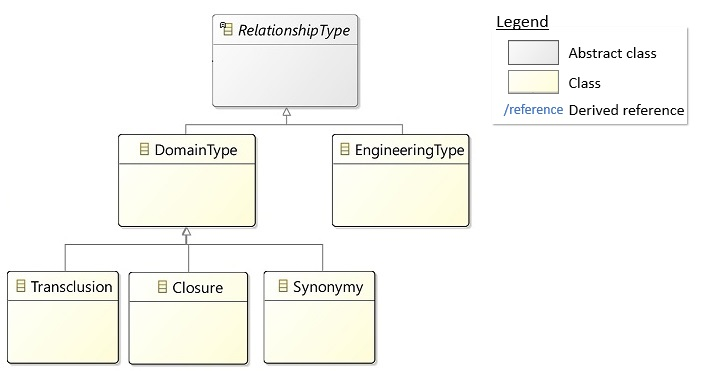
\includegraphics[width=.8\linewidth]{images/relationtyping-re-mm.jpg}
	\caption{Customized relationship typing tailored to transclusion.}
	\label{fig:mm-relationtyping-re-mm}
\end{figure}







